\chapter{Best Things about MTJs}


\section{Critical Voltage Measurement}




\section{Field Modulated Mag-noise Measurement}


The UCI group developed a novel method of experimental characterization of the spectrum of spin wave eigenmodes of individual STT-MRAM elements. This method is magnetic noise spectroscopy with magnetic field modulation. Figure 3(a) shows the experimental setup for measuring magnetic noise with magnetic field modulation, in which a microwave-frequency noise emitted by the STT-MRAM at a finite bias current is measured via a lock-in detection

\begin{figure}[!ht]
  \centering
  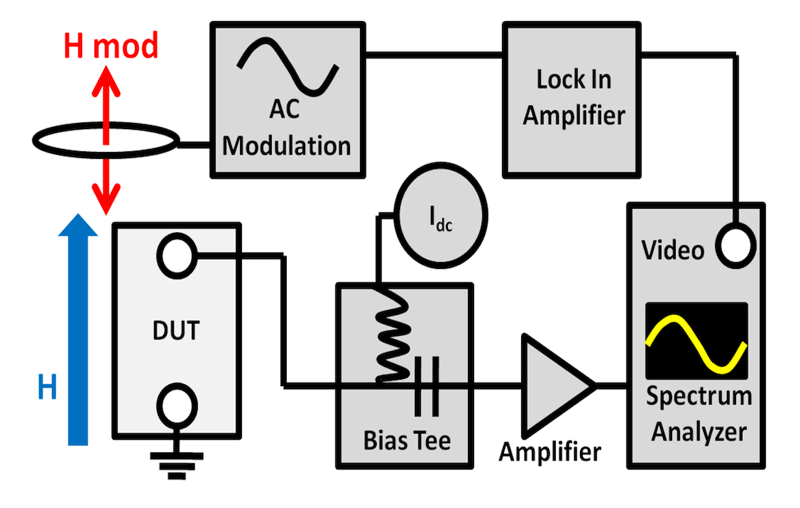
\includegraphics[width=0.6\textwidth]{fig/magnoise/Picture1.png}
   \caption{Set-up for Magnoise measurement}
  \label{fig:magnoise-setup}
\end{figure}

technique. The microwave noise is emitted at the frequencies of spin wave eigenmodes of the sample, with the most prominent features arising from spin wave eigenmodes of the free layer. The top panel of Figure 3(b) shows the magnetic noise spectrum measured by conventional technique without magnetic field modulation. The conventional method only allows us to reliably measure the frequency of the quasi-uniform spin wave mode. 






In contrast, the data obtained with magnetic field modulation shown below allow us to detect not only the resonant frequencies but also the spectral linewidth of several spin wave modes of the device. This is enabled by the superior signal-to-noise factor of our technique with magnetic field modulation. The data obtained with magnetic field modulation is of high enough quality to enable determination of the Gilbert damping, magnetic anisotropy and exchange stiffness constant of the free layer. The main feature of the magnetic noise method is that it allows measurement of the spin wave spectrum faster than the ST-FMR method.  Therefore, this method can be used for rapid screening of magneto-dynamic properties of STT-MRAM cells.




\begin{figure}[!ht]
  \centering
  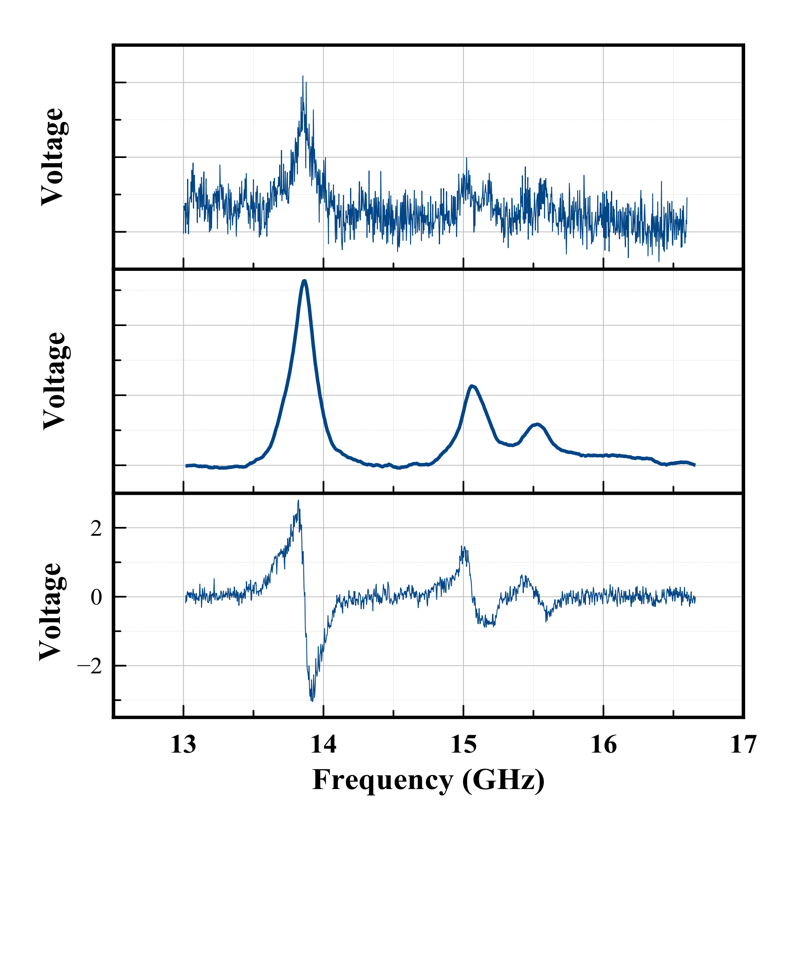
\includegraphics[width=0.6\textwidth]{fig/magnoise/magnoise-data.png}
   \caption{Set-up for Magnoise measurement}
  \label{fig:magnoisedata}
\end{figure}



\section{Comparison between Magnoise and ST-FMR technique }